%!TEX root = ../document.tex
\chapter{Project Plan}

This project will follow the system implementation methodology summarized by the company in the field of manufacturing system implementation. The project will follow this implementation methodology.

\section{Project phases and key tasks}

According to the implementation methodology, the whole process of the project is devided into 4 following phases.

\begin{itemize}
	\item \textbf{Project preparation} --- \textit{Object definition}

	\item \textbf{Blue print design} --- \textit{Target decomposition}

	\item \textbf{Manufacturing} --- \textit{Aims achieved}

	\item \textbf{Acceptance of delivery} --- \textit{Customer value realization}
\end{itemize}

Each step of the four-step implementation method is divided into tasks in detail, and the specific work content, work time, work mode, person in charge and work results of each step are defined.

The following page are the work breakdown structure(WBS) of the project.

\begin{landscape}

\begin{center}
\Large \textbf{Work Breakdown Structure(WBS) of the project}     

\begin{figure}[!htb]
\centering
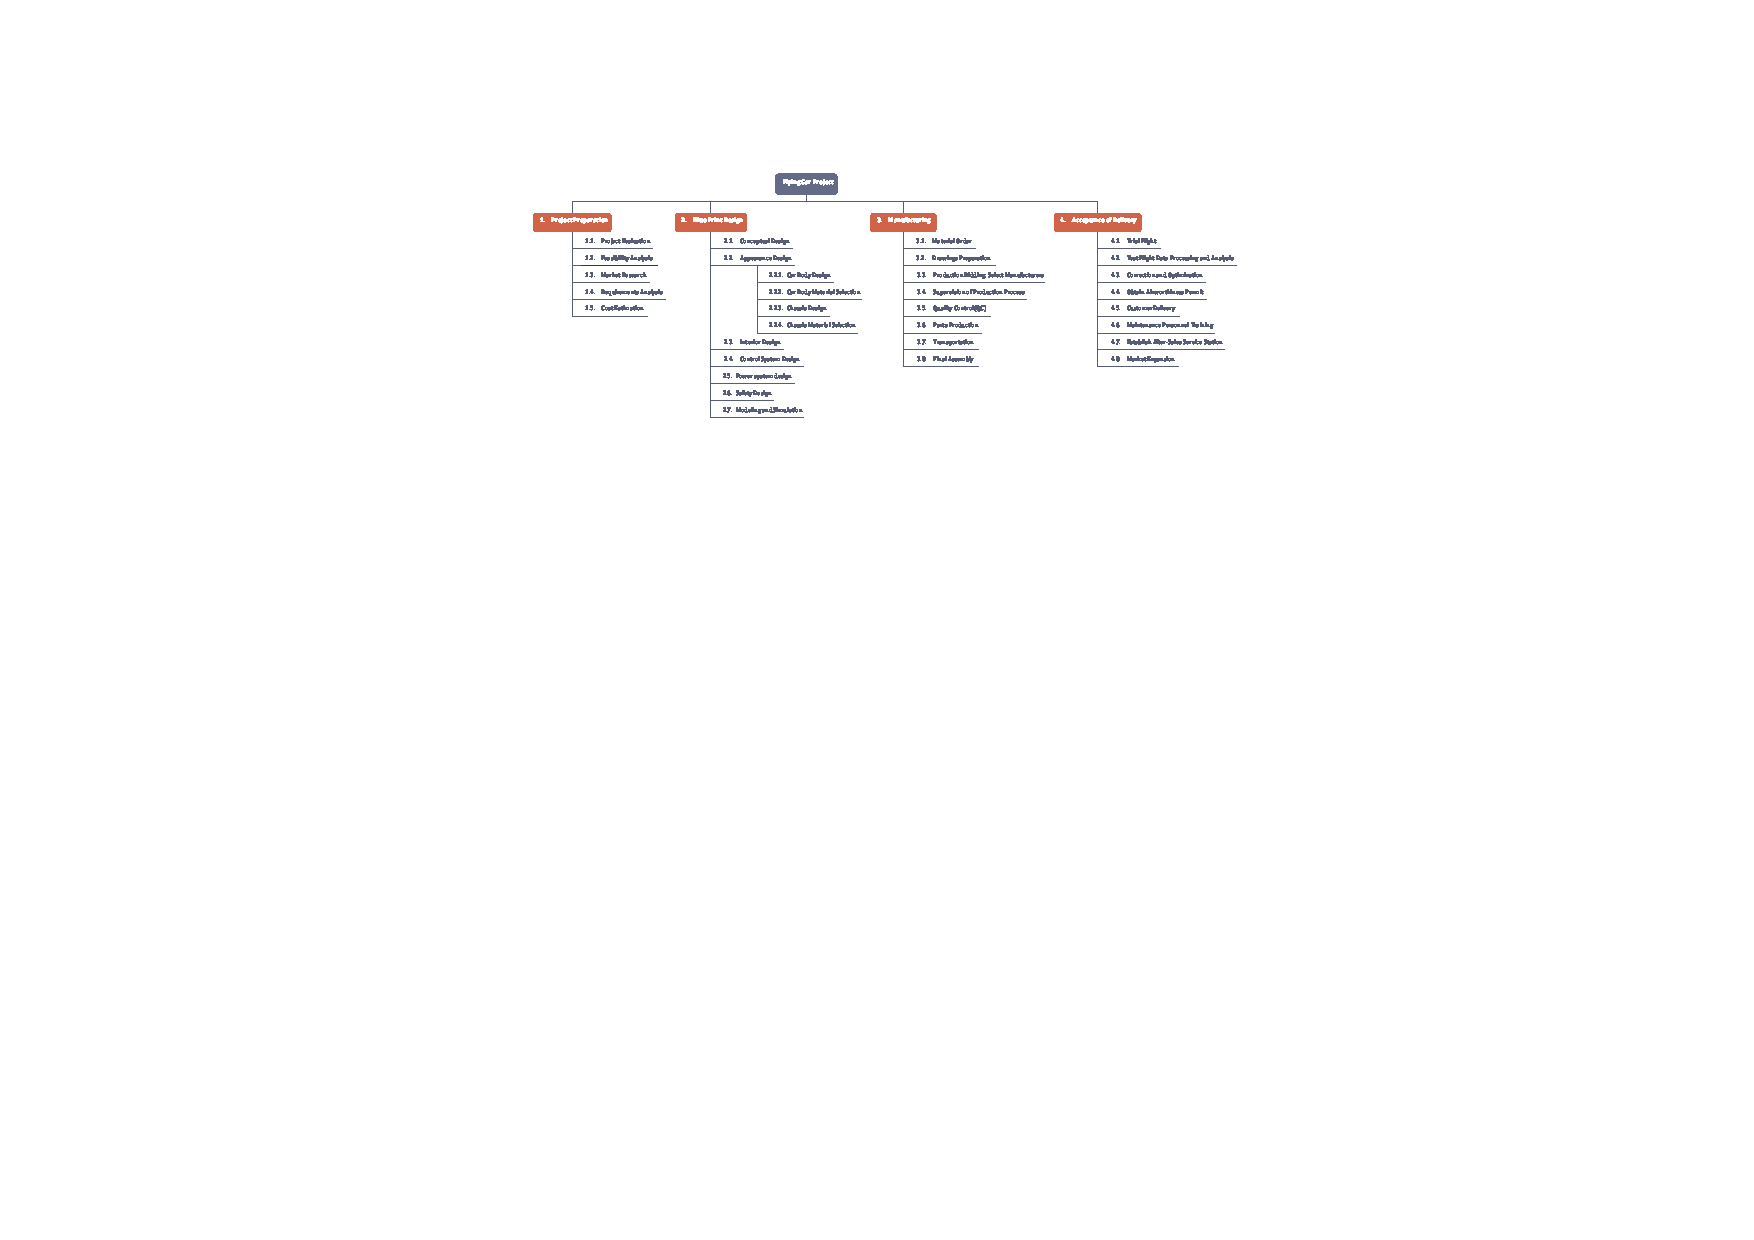
\includegraphics[angle=-90,width=25cm]{pic/wbs.pdf}
% \caption{WBS}
% \label{fig:wbs}
\end{figure}

\end{center}

\end{landscape}

\section{Timeline}

According to the above implementation methodology, the specific implementation plan of this project is as follows, and the project work will be carried out according to this plan. The planned whole life cycle of the project is 16 years until 2035. 

The following page shows the Gantt chart of the project.

\section{Milestone}

A milestone is a point in time used to mark the events or major accomplishments of the project team, as well as to mark the progress of the project. The major milestones and associated timelines for the Flying Car project are as follows:

\renewcommand\arraystretch{1.8}
\begin{table}[!htb]
\centering
\footnotesize
\begin{tabular}[b]{|p{4cm}<{\raggedright}|p{6cm}<{\raggedright}|p{4cm}<{\raggedright}|}
\hline
\textbf{Project phase} & \textbf{Milestone} & \textbf{Planned date} \\
\hline
\multirow{3}{*}{\bfseries \footnotesize Project preparation} &  Officially approved &   \\
\cline{2-3}
                         &  Reliability analysis completed &   \\
\cline{2-3}
                         &  Market survey completed  &   \\
\cline{2-3}
                         &  Cost estimates, budget allocations &   \\
\hline
\multirow{3}{*}{\bfseries \footnotesize Blue print design} &  Establish a design team &   \\
\cline{2-3}
                         &  Completion of Concept selection &   \\
\cline{2-3}
                         &  Completion of pneumatic design &   \\
\cline{2-3}
                         &  Completion of overall design &   \\
\cline{2-3}
                         &  Completion of simulation experiment &   \\                         
\cline{2-3}
                         &  Safety verification &   \\
\hline
\multirow{3}{*}{\bfseries \footnotesize Manufacturing} &  Production Bidding, Select Manufactures &   \\
\cline{2-3}
                         & Assembly completed, prototype offline  &   \\
\hline
\multirow{3}{*}{\bfseries \footnotesize Acceptance of delivery} &  First trial flight &   \\
\cline{2-3}
                         &  Obtain Airworthiness Permit &   \\
\cline{2-3}
                         &  CustomerDelivery &   \\
\cline{2-3}
                         &  Market Expansion &   \\
\hline
\end{tabular}
\end{table}

\begin{landscape}

\begin{center}
\Large \textbf{Gantt chart(Timeline) of the project}   

\begin{figure}[!htb]
\centering
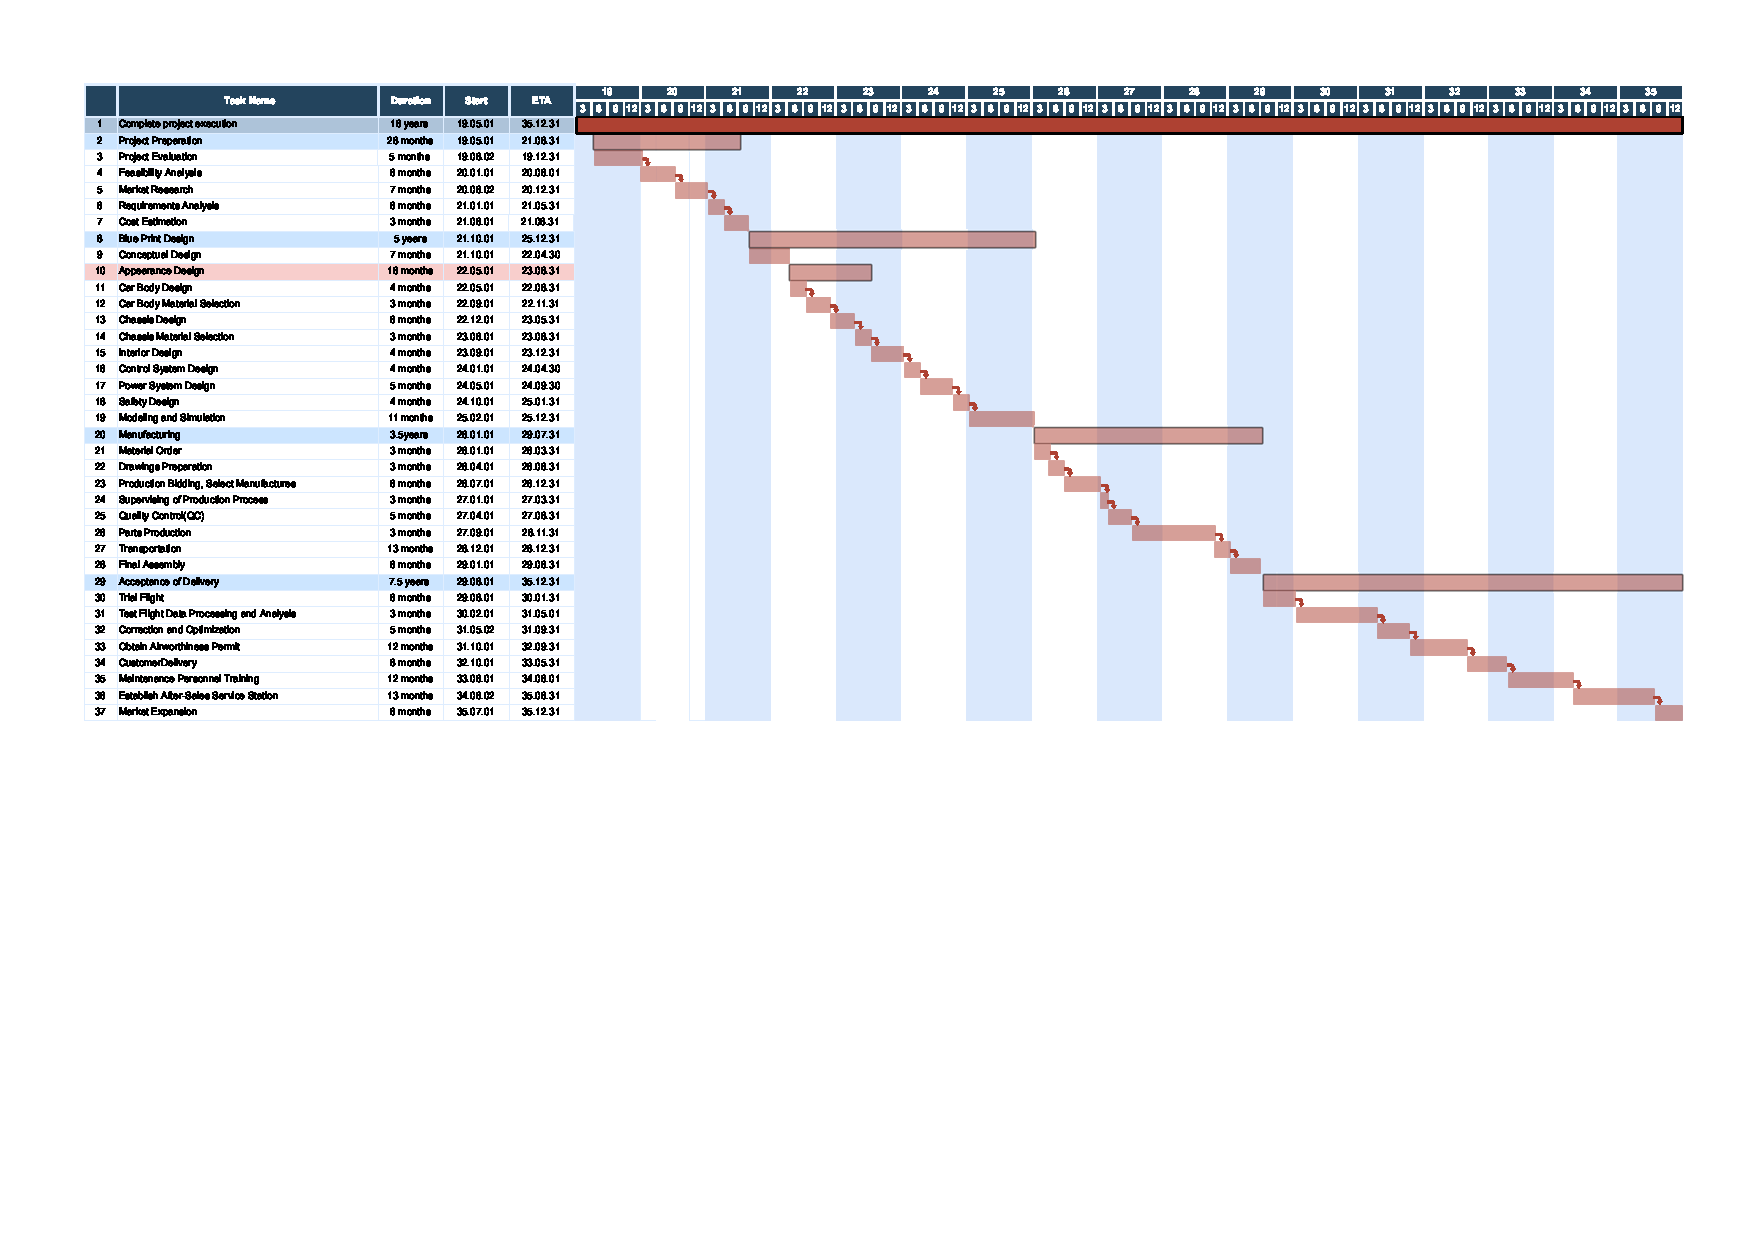
\includegraphics[angle=-90,width=25cm]{pic/gantt.pdf}
% \caption{WBS}
% \label{fig:wbs}
\end{figure}

\end{center}

\end{landscape}

\section{Project plan execution and report}

The project manager is primarily responsible for monitoring the progress of the project. The project plan is the key document used to inform the progress and current status of the project. The project plan includes project phase, task, duration, resources, scheduled start and end dates, milestones, persons responsible, and deliverables. The Project plan will be maintained by \textbf{XXX} and will reflect the Project methodology planning phase.

Only in two cases can the entire baseline plan be redesigned. One is that the entire baseline plan should be updated whenever there is any scope change that fundamentally affects project progress. Similarly, when schedule or budget deviations are significant, benchmark plans need to be reworked to make performance reports meaningful again.

The execution and reporting of the project plan shall be carried out in accordance with the following procedures: each project team member shall be responsible for updating the actual progress according to the project plan and estimating how long it will take to complete the tasks assigned to him/her as part of the weekly project report meeting. The project management team meets every Friday to review project progress against the project plan. The review is based on a review of delays, focusing on identifying existing or potential task delays, assessing the impact on the project, and agreeing on action plans to be taken to mitigate the impact. Project managers highlight tasks that may be delayed (e.g., expected completion time is later than planned). The person in charge of the task should develop an action plan for potential delays to minimize the impact on other project work. The project team leader shall indicate the possible task delay in the problem section of the weekly status report, including a brief description of the problem, a brief description of the action plan to prevent the delay or the date of the new task, and the date shall indicate the impact on other tasks.